% -*- coding: utf-8 -*-
\documentclass[11pt]{oblivoir}
\usepackage[utf8]{inputenc}
\usepackage{kotex}
\usepackage[scale=0.75, bindingoffset=5mm, a4paper]{geometry}
\usepackage{indentfirst}
\usepackage{graphicx}
\usepackage{color}
\usepackage{background}

\backgroundsetup{contents=
\includegraphics{Pictures/sunrin.png}, opacity=0.2, scale=1, angle=270}

\newenvironment{textbox}
	{
	\begin{center}
		\begin{tabular}{|p{0.95\textwidth}|}
			\hline
	}
	{
		\\ \hline
		\end{tabular}
		\end{center}
	}

\title{\textbf{엔씨소프트 분석을 통한 기업 전망 예측 및 발전 방안 연구}}
\author{\textbf{1학년 9반 15번 박태원}}

\begin{document}
	\begin{center}
		\maketitle
		\begin{abstract}
			아직 쓸 요약이 없노
		\end{abstract}
		\tableofcontents
		\pagebreak
	\end{center}
	
	\backgroundsetup{contents=""}
	
	\section{서론}
		\subsection{선정 배경 및 목적}
			\textbf{게임 엔터테인먼트 산업}은 4차 산업혁명의 역풍에 굴하지 않고 꾸준히 각광받고 있는 산업으로, 국내 시장에서는 2015년 최초로 \textbf{10조 원} 이상의 매출액을 기록한 이후 `16년에는 \textbf{11조 원}, `17년에는 \textbf{12조 원}, 가장 최근인 `18년에는 \textbf{13조 원}을 기록하며 지속적인 성장세를 보여주고 있다.\footnote{콘텐츠산업 2018년 결산 및 2019년 전망 보고서 34p}
			
			\begin{figure}[htbp]
				\centering
				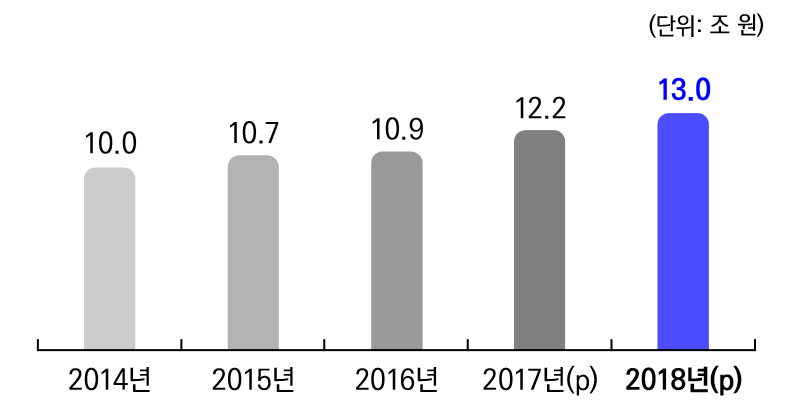
\includegraphics[width=0.7\textwidth]{Pictures/GameMaechul.png}
				\caption{게임 산업 매출액 추이}
			\end{figure}
			
			또한 최근에는 \textbf{E-SPORTS 산업}의 성장으로 인해 \textbf{2020년까지 꾸준히 상승}할 것으로 전망되었으며, \footnote{한국콘텐츠진흥원 대한민국 게임백서 2018 6p} 
			\textbf{VR 기술}의 비약적인 발전과 \textbf{모바일 게임} 시장의 확대로 인하여 앞으로의 발전 가능성이 높은 산업이라 여겨지고 있다.
			
			이러한 게임 산업의 발전으로 인하여 게임 시장의 중요성은 날로 부각되어가고 있는 추세이다. 따라서 \textbf{IT 경영과}에 재학 중인 학생으로서 IT 시장의 신흥 강자로 떠오르고 있는 \textbf{게임 시장}을 분석해보는 것은 4차 산업혁명을 이해하고 대비하는 과정에 있어서 무척이나 도움이 될 것이라 판단하게 되었다.
			
			그중에서도 이번 연구 대상으로 선정된 \textbf{"엔씨소프트"}는 국내에서 오랜 세월 명목을 이어오고 있는 게임 개발사 중 하나이며, 한때 온라인 게임계에 이름을 휘날렸던 \textbf{"아이온"}과 대한민국 게임계에 한 획을 그었다고 평가받는 \textbf{"리니지"} 시리즈를 개발하여 대한민국 게임 시장에 지대한 영향을 미치고 있는 기업이기도 하다. 
			
			이에 대한 통계로, 게임 퍼블리셔를 기준으로 정렬한 \textbf{2019년 상반기 모바일 게임 매출 점유율}을 들 수 있다. 다음은 그것을 도식화 한 것이다
			\footnote{MOBILEINDEX 2019년도 상반기 한국 모바일 게임 시장 총정리 6p}:
			
			
			\begin{figure}[htbp]
				\centering
				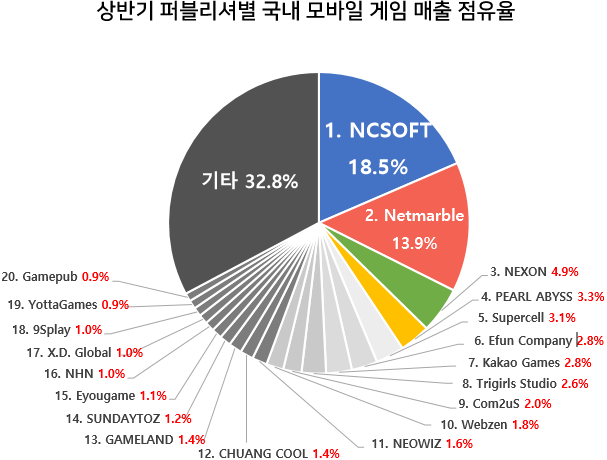
\includegraphics[width=0.8\textwidth]{Pictures/MobileMaechul.png}
				\caption{2019년도 상반기 모바일 게임 매출 점유율 (퍼블리셔별)}
			\end{figure}
			
			이러한 관점에서 엔씨소프트가 \textbf{게임 엔터테인먼트 기업의 표본}으로서 적절한 뿐 만 아니라, 그 경영 전략을 분석하고 연구하기에도 상당히 가치 있는 기업이라 판단하게 되었다.
			
			이에 본 논문에서는 엔씨소프트를 분석함으로서 기업의 비전과 경영 방법이 실적에 미친 영향에 대하여 제시하고자 하며, 궁극적으로는 학과에서 주어진 연구 목적을 달성하기 위하여 결론으로서 \textbf{기업 전망 예측}과 \textbf{발전 방안}을 제시하고자 한다.
					
		\subsection{방법}
			서론을 제외한 본문이 시작되는 2장에서는 심화 분석의 원활한 진행을 위하여 선행 조사를 실시하였다. 선행 조사는 \textbf{기업 개요, 기업 연혁, 기업 비전} 총 3개의 주제로 이루었으며, \textbf{엔씨소프트 공식 홈페이지\footnote{http://kr.ncsoft.com/korean/}}에서 소개하고 있는 자사의 개요, 
			연혁, 비전을 활용하는 것으로 하였다. 
			
			3장에서는 선행 조사를 통하여 수집된 자료들을 기반으로 \textbf{시장, 환경, 경쟁사, 마케팅}의 방면에서 분석하였다. 또한 다시 이를 기반으로 경영 실적을 확인하기 위해 \textbf{재무, 주식}에 관하여 분석하였다. 분석용 자료로서는 \textbf{확인된 보도자료, 엔씨소프트 공식 발표 자료, 네이버 금융}을 활용하여 자료의 신뢰성을 확보하였다.
			
			4장에서는 심화 분석 결과를 요약하고, 이를 토대로 하여 \textbf{기업 전망 예측}과 \textbf{발전 방안}을 제시하였다.
			\begin{figure}[htbp]
				\centering
				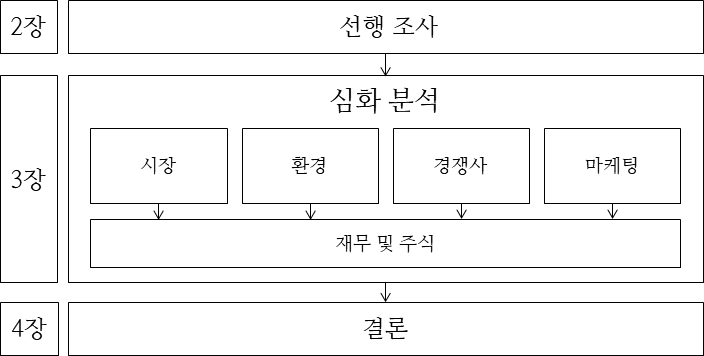
\includegraphics[width=1\textwidth]{Pictures/Methods.png}
				\caption{연구 구성}
			\end{figure}
			
	
	\section{선행 조사}
		\subsection{기업 개요}
		\noindent 
		\footnote{http://kr.ncsoft.com/korean/aboutus/overview.aspx, [엔씨소프트 공식 홈페이지 - 기업 개요 캡쳐]}
		\begin{figure}[htbp]
			\centering
			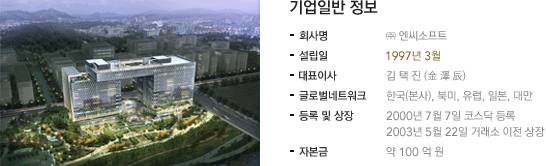
\includegraphics[width=1\textwidth]{Pictures/ncinfo.png}
			\caption{엔씨소프트 일반 정보}
		\end{figure} 
		
		엔씨소프트는 \textbf{게임 개발 및 배급}을 주 업무로 삼고 있으며, 1998년 \textbf{리니지}를 시작으로 인터넷 기반 온라인 게임의 대중화를 이끌었다. 또한 해외 시장을 개척, 아시아, 북미, 유럽 등에 \textbf{글로벌 네트워크}를 확보해 나가고 있다.
		
		엔씨소프트는 본래 창업 당시인 1997년 \~ 1999년까지는 온라인 게임 전문이 아닌 인터넷 기반 기업용 소프트웨어 개발 업체였다. 김택진 CEO가 송재경의 리니지 팀을 인수하여 정식 서비스를 개시한 후, 리니지의 대성공을 발판으로 다른 사업을 정리하고 본격적인 게임 사업에 뛰어들게 되었다.\footnote{[인물열전] '바람의나라' 와 '리니지' 의 아버지, 송재경 - 게임메카}
		
		작은 개발사를 인수하여 게임을 서비스하는 타 배급사와는 다르게 대부분의 게임을 자사에서 직접 개발하여 서비스하며, 한때 캐주얼 게임에 진출하려 시도한 적이 있었으나 대차게 망하고 온라인 RPG에 주력하고 있다.
		
		\subsection{기업 연혁}
			다음은 엔씨소프트에서 공개하고 있는 연혁 중, 기업의 경영 실적에 영향을 끼쳤으리라 예상되는 부분을 정리한 것이다.
			\begin{textbox}
			\textbf{\textcolor{blue}{1997. 3}} 엔씨소프트 창립
			\\
			\textbf{\textcolor{blue}{1998. 9}} 게임  \textbf{리니지} 상용서비스 개시
			\\
			\textbf{\textcolor{blue}{2000. 5}} 글로벌 네트워크 구축개시 (해외법인)
			\\
			\textbf{\textcolor{blue}{2000. 7}} 해외 서비스 개시 (리니지 대만 서비스 시작)
			\\
			\textbf{\textcolor{blue}{2000. 7}} 코스닥 등록(2003년 한국증권거래소로 이전 상장)
			\\
			\textbf{\textcolor{blue}{2003. 10}} 게임 \textbf{리니지2} 서비스 개시
			\\
			\textbf{\textcolor{blue}{2005. 4}} \textbf{길드워} 상용서비스 개시 (북미 / 유럽 시장)
			\\
			\textbf{\textcolor{blue}{2008. 5}} 엔씨소프트 R\&D(Research \& Development) 센터 완공
			\\
			\textbf{\textcolor{blue}{2008. 11}} 게임 \textbf{아이온} 서비스 개시
			\\
			\textbf{\textcolor{blue}{2009.}} 게임 \textbf{아이온} 글로벌 론칭
			\\
			\textbf{\textcolor{blue}{2012. 6}} 게임 \textbf{블레이드 \& 소울} 서비스 개시
			\\
			\textbf{\textcolor{blue}{2012. 8}} 게임 \textbf{길드워 2} 상용서비스 개시
			\\
			\textbf{\textcolor{blue}{2013. 8}} 판교 R\&D 센터 완공
			\\
			\textbf{\textcolor{blue}{2014. 6}} 게임 \textbf{와일드스타} 북미/유럽 상용서비스 개시
			\\
			\textbf{\textcolor{blue}{2015. 5}} 북미법인 엔씨웨스트(NC West)의 모바일 스튜디오 설립
			\\
			\textbf{\textcolor{blue}{2015. 10}} 게임 \textbf{길드워2: 가시의 심장} 상용서비스 개시
			\\
			\textbf{\textcolor{blue}{2016. 1}} 게임 \textbf{블레이드 \& 소울} 북미/유럽 정식 서비스 돌입
			\\
			\textbf{\textcolor{blue}{2016. 12}} 게임 \textbf{리니지 레드나이츠} 아시아 12개국 정식 서비스
			\\
			\textbf{\textcolor{blue}{2017. 6}} 게임 \textbf{리니지 M} 서비스 개시
			\\
			\textbf{\textcolor{blue}{2017. 6}} 게임 \textbf{MXM} 북미/유럽 출시
		\end{textbox}
		\pagebreak
		\subsection{기업 비전 및 사명}
			엔씨소프트는 기업의 주요 비전을 \textbf{Mission, Format, Core Value, Spirit} 총 4가지로 분류하였다. 
			\begin{figure}[htbp]
				\centering
				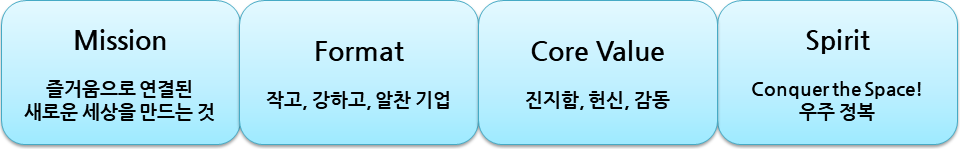
\includegraphics[width=1\textwidth]{Pictures/vision.png}
				\caption{엔씨소프트 기업 비전}
			\end{figure}

			\textbf{Mission}은 엔씨소프트가 이루고자 하는 사명으로, 온라인을 넘어 즐거움으로 연결된 세상을 만들겠다는 결연한 의지를 나타내고 있다.
			
			\textbf{Format}은 \textbf{작고, 강하고, 알찬 기업} 3가지 의미로 나뉜다. 
			\textbf{작다}는 존중을 바탕으로 하나의 팀으로서의 커뮤니케이션이 이루어지는 회사를 의미한다. \textbf{강하다}는 바르게 결정하고 전체가 움직이는 것을 의미한다. \textbf{알차다}는 선택과 집중을 통해 잘하는 일은 누구보다 탁월하게 잘하여 감동을 창조하겠다는 비전을 나타낸다.
			
			\textbf{Core Value}는 기업의 핵심 가치로, \textbf{진지함, 헌신, 감동} 3가지 의미로 나뉜다. \textbf{진지함}은 도덕적, 또는 예술적 가치에 집착하고, 자신이 하는 일에 진지하게 임하겠다는 것을 의미한다. \textbf{헌신}은 엔씨소프트가 스스로 하는 일에 대한 눈부신 열정, 그 열정이 헌신이라 여겨질 정도로 일에 대해 열정을 갖겠다는 것을 의미한다. \textbf{감동}은 사소한 불편을 제거하고자 끊임없이 개선하고, 한 걸음 한 걸음 디테일을 조각해 내어 사람들을 감동시킬 때까지 노력하겠다는 의지를 의미한다.
			
			\textbf{Spirit}은 기업 정신으로, \textbf{Conquer the Space! 우주 정복}이라는 문장으로 표현할 수 있다. 이는 남들이 만들려는 것을 똑같이 개발하려는 것이 아니라, 항상 자신이 꿈꾸는 새로운 세계를 만들어나가야 한다는 엔씨소프트의 정신을 담은 문장이다. 남들이 가지 않은 별을 찾아서 \textbf{'감동'}을 주겠다는 것이 정복의 의미이다.

		\subsubsection{기업 CI}
			\begin{figure}[htbp]
				\centering
				
\includegraphics[width=0.8\textwidth]{Pictures/ci.png}
				\caption{엔씨소프트 기업 CI}
			\end{figure}
			
			로고와 회사 명에 포함되어 있는 'NC'는 창업 당시 Next Company의 의미를 담고 시작했다고 한다. 뜻은 단순히 회사 이름을 정하지 못했던 탓이었다고 한다. 하지만 이내 '영화를 뛰어넘는 게임을 만들자'는 의미에서 'Next Cinema'의 준말로 바뀌게 되었고, 현재에는 다시금 \textbf{'끊임없이 변화하는 회사가 되자'}라는 의미를 담아 \textbf{'Never ending Change'}의 준말로 바뀐 상태이다.
			
			엔씨소프트의 CI는 \textbf{혁신적인 변화와 성장의 의미}를 담고 있으며, 현재에 만족하지 않고 항상 도전하며 끊임없이 창의를 추구하는 엔씨인의 정신을 형상화 한 것이다. N과 C의 연결을 통한 공간과 입체형태는 \textbf{엔씨소프트와 고객이 즐거움으로 연결되는 새로운 세상의 창조}를 의미한다.
			
			또한 엔씨소프트의 기업 컬러로서, 우아함과 완결을 의미하는 \textbf{'골드'}, 견고함과 신뢰를 의미하는 \textbf{'다크블루'}, 순수함과 무한을 의미하는 \textbf{'순백색'}을 하나로 모아 창의적이며 미래지향적인 기업 정체성을 반영하였다.
			
	\section{본론}
		\subsection{시장 분석}
		\noindent
		다음은 2019년 상반기 매출 상위 7개 모바일 게임을 정리한 도표이다.  \footnote{MOBILEINDEX 2019년 상반기 한국 모바일 게임 시장 총정리 9p}
		\begin{figure}[htbp]
			\centering
			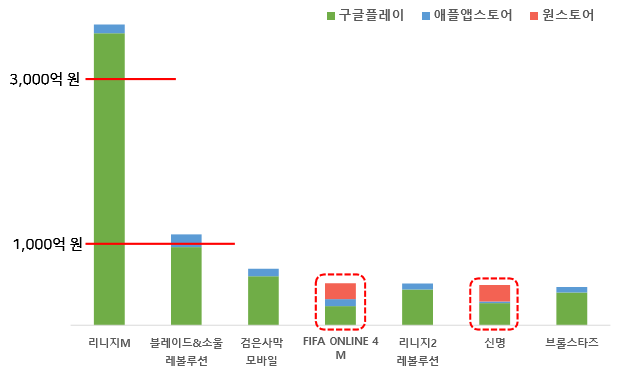
\includegraphics[width=0.9\textwidth]{Pictures/Sangbangi.png}
			\caption{2019년 상반기 매출 TOP7 모바일 게임}
		\end{figure}
		
		\textbf{상위 매출 모바일 게임 1위}가 엔씨소프트의 \textbf{리니지M}이다. \textbf{리니지M}은 엔씨소프트가 개발과 배급을 모두 담당하였다. 연혁에서 확인할 수 있듯이, 리니지 M은 2017년 출시된 게임으로 올해 뿐 만 아니라, \textbf{출시 이후 2년 연속 매출 1위}를 기록하고 있다.
		\footnote{http://www.thegames.co.kr/news/articleView.html?idxno=212779, '리니지 M' 2년 연속 매출 1위 '맹렬 질주'}
		매출 2위와 매출 3위의 점유율을 합쳐도 리니지M의 점유율에 미치지 못한다. 심지어 매출 2위인 블레이드\&소울 레볼루션의 IP는 본래 엔씨소프트의 것이다.
		
		 \begin{figure}[htbp]
		 	\centering
		 	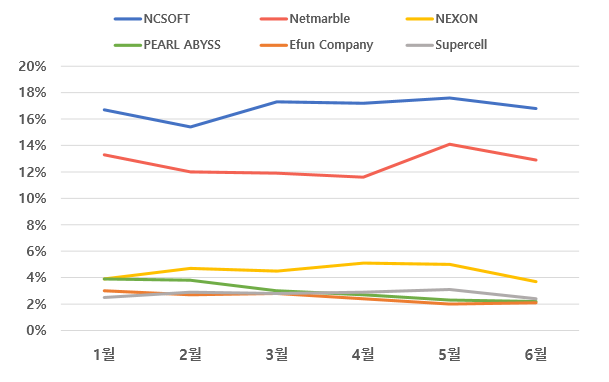
\includegraphics[width=0.8\textwidth]{Pictures/PublisherMaechul.png}
		 	\caption{2019년 상반기 퍼블리셔별 매출 점유율}
		 \end{figure}
	 
	 	또한 위의 게임 배급사 별 매출 점유율을 보면, 엔씨소프트가 거의 전체의 약 16\~18\%의 지분을 가지고 있는 것을 확인할 수 있다. 심지어 작년에는 \textbf{리니지 2 레볼루션}과 
	 	\textbf{리니지M}이 18년도 하반기 구글플레이 시장 규모를 \textbf{2배 가까이} 늘려놓아 \textbf{한국 구글 플레이 연도별 누적 매출 최초 3조 돌파}라는 실적을 달성할 수 있었다.\footnote{https://www.mk.co.kr/news/it/view/2017/12/821784/, ‘리니지의 힘’ 韓 구글 플레이 사상 최초 누적매출 3조 돌파} 모바일 게임 시장이 대세인 현재, 그것도 모바일 게임 시장에서 가장 큰 영향력을 가지고 있는 구글플레이의 매출을 들었다 놓았다 하는 것을 보면 엔씨소프트의 시장 영향력은 가히 어마어마하다고 할 수 있다. 
	 	
		\subsection{환경 분석}
		
		환경 분석으로는 SWOT 분석과 PEST 분석을 진행하였다. 
		
		\begin{figure}[htbp]
			\centering
			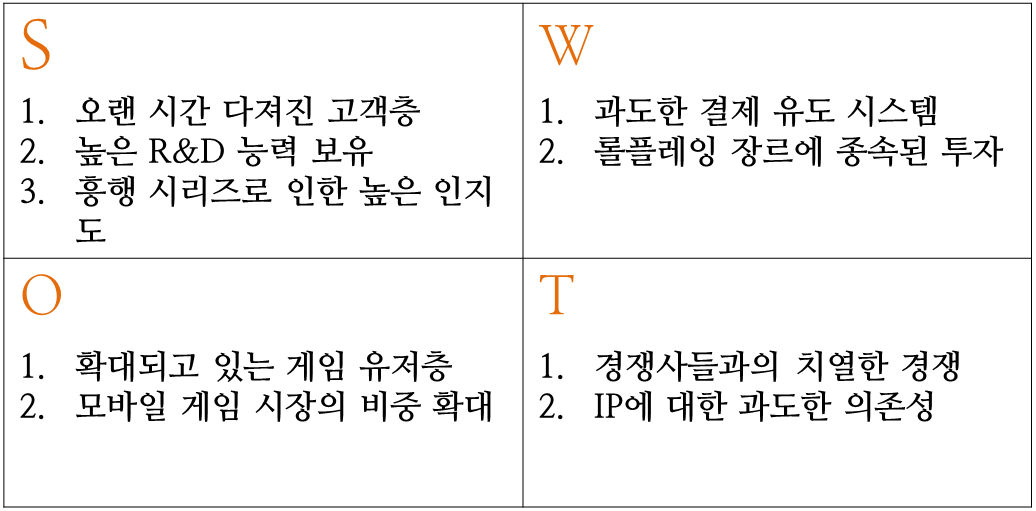
\includegraphics[width=1\textwidth]{Pictures/SWOT.png}
			\caption{엔씨소프트 SWOT 분석}
		\end{figure}

	
	
		\subsection{경쟁사 분석}
		
		\subsection{마케팅 분석}
		
		\subsection{재무 분석}
		
		\subsection{주가 분석}
	
	\section{결론}
	
	\section{레퍼런스}
	

\end{document}